\documentclass{article}
\usepackage{geometry}
 \geometry{
 a4paper,
 total={170mm,270mm},
 left=20mm,
 top=10mm,
 }
\usepackage{graphicx}
\usepackage{float}
\usepackage{enumitem}
\usepackage{caption}
\usepackage{amsmath}
\usepackage{datetime}
\usepackage{multirow}
\usepackage{listings}
 
\newcommand\blfootnote[1]{%
  \begingroup
  \renewcommand\thefootnote{}\footnote{#1}%
  \addtocounter{footnote}{-1}%
  \endgroup
}

\newdate{date}{06}{09}{2016}
\date{\displaydate{date}}
\title{\textbf{Network Analysis and Modelling - CSCI 5352} \\
Problem Set 1}
\author{\textbf{Santhanakrishnan Ramani}}
\begin{document}
\maketitle

\section*{Problem 1}
\begin{enumerate}[label=(\alph*)]
\item
The adjacency matrix of network (A) is

\begin{tabular}{l r|l l l l l}                      
& \multicolumn{1}{r|}{A} &1   &2   &3   &4   &5   \\ \cline{2-7}
& \multicolumn{1}{r|}{1} &0   &1   &0   &0   &1   \\
& \multicolumn{1}{r|}{2} &0   &0   &1   &0   &0   \\ 
& \multicolumn{1}{r|}{3} &1   &0   &0   &0   &0   \\
& \multicolumn{1}{r|}{4} &1   &0   &0   &0   &1   \\ 
& \multicolumn{1}{r|}{5} &0   &0   &1   &1   &0   \\ 
\end{tabular}

\item
The adjacency list of network (A) is \bigskip \\ 
\begin{minipage}[b]{0.4\textwidth}
\underline{A\hspace{1.5cm}}\\
1 $\rightarrow$ \{2,5\}\\
2 $\rightarrow$ \{3\}\\
3 $\rightarrow$ \{1\}\\
4 $\rightarrow$ \{1,5\}\\
5 $\rightarrow$ \{3,4\}
\end{minipage}

\item
Adjacency matrices of One Mode Projections of Network (B) are \bigskip \\ 

\begin{minipage}[b]{0.4\textwidth}
    \begin{tabular}{l r|l l l l l}                      
		& \multicolumn{1}{r|}{A} &1   &2   &3   &4   &5   \\ \cline{2-7}
		& \multicolumn{1}{r|}{1} &0   &1   &1   &1   &1   \\
		& \multicolumn{1}{r|}{2} &1   &0   &0   &1   &1   \\ 
		& \multicolumn{1}{r|}{3} &1   &0   &0   &0   &0   \\
		& \multicolumn{1}{r|}{4} &1   &1   &0   &0   &0   \\ 
		& \multicolumn{1}{r|}{5} &1   &1   &0   &0   &0   \\ 
	\end{tabular}
\end{minipage}
\hfill
\begin{minipage}[b]{0.4\textwidth}
    \begin{tabular}{l r|l l l l l l}                      
		& \multicolumn{1}{r|}{A} &1   &2   &3   &4   &5  &6 \\ \cline{2-8}
		& \multicolumn{1}{r|}{1} &0   &1   &1   &0   &1  &0\\
		& \multicolumn{1}{r|}{2} &1   &0   &1   &0   &0  &1\\ 
		& \multicolumn{1}{r|}{3} &1   &1   &0   &1   &1  &0\\
		& \multicolumn{1}{r|}{4} &0   &0   &1   &0   &0  &0\\ 
		& \multicolumn{1}{r|}{5} &1   &0   &1   &0   &0  &0\\ 
		& \multicolumn{1}{r|}{6} &0   &1   &0   &0   &0  &0\\ 
	\end{tabular}
\end{minipage}
\end{enumerate}

\section*{Problem 2}
Given, \textbf{A} the adjacency matrix of a simple graph and \textbf{1} the column vector whose elements are all 1
\begin{enumerate}[label=(\alph*)]
\item
The vector \textbf{K} whose elements are the degrees $k_i$ of the vertices is given by
$$K = A . 1$$
As the row sum of the adjacency matrix gives the degree of the node corresponding to that row.

\item
The number \textit{m} of edges in the network is,
$$m = \dfrac{1}{2} (A . 1) 1^T$$
Since it's a simple graph, the number of edges is half the sum of degrees of all the nodes in the graph.

\item
The matrix \textbf{N} whose elements $N_{ij}$ is equal to the number of common neighbour of vertices i and j is
$$N = A  A^T$$ 
There will be a common neighbour for vertices i and j only if there is a vertex k such that $A_{ik} = A_{kj} = 1$

\item
Total number of triangles in the network are,
$$Traingle\_Count = \dfrac{1}{6} * Tr((A  A^T)A)$$
Since, $A A^T$ gives the number of common neighbours of vertices i and j, triangles could be formed if there is an edge between i and j.
\\As it's a simple graph, each edge is considered 2 times, and each of the 3 vertices forming the triangle adds up individually, the triangle count is found out by taking the trace of common neighbours and adjacency matrix and dividing it by 6 (2*3). 
\end{enumerate}

\section*{Problem 3}
Given a bipartite graph with $n_1$ vertices of type 1 and $n_2$ vertices of type 2, prove that the mean degrees $c_1$ and $c_2$ of the two types are given by,
$$ c_2 = \dfrac{n_1}{n_2} c_1$$

Proof:\\

As the graph is bipartite, there can be edges only between two nodes of different type, therefore
\begin{equation} \label{eq:1}
\text{Mean degree } c_1 \text{ of type 1} = \dfrac{\text{No of edges in the graph}}{n_1}
\end{equation}

\begin{equation} \label{eq:2}
\text{Mean degree } c_2 \text{ of type 2} = \dfrac{\text{No of edges in the graph}}{n_2}
\end{equation}

\begin{center}
From (\ref{eq:1}) and (\ref{eq:2}), we can see that, $c_2 = \dfrac{n_1}{n_2} c_1$ 
\end{center}


\section*{Problem 4}
\begin{enumerate}[label=(\alph*)]
\item
K-core network is obtained by repetitively removing nodes whose degree are less than K. In the end we are left with the subset of graph whose vertices have a minimum degree of K. 3-core in network (A) is, 
\begin{figure}[!h]
  \centering
  \begin{minipage}[b]{0.3\textwidth}
    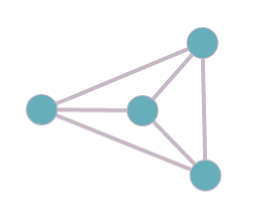
\includegraphics[width=\textwidth]{images/4a1.png}
  \end{minipage}
\end{figure}

\item
Reciprocity (r) of a network is given by the formula,
$ r = \dfrac{1}{m} Tr(A^2)$
where A is the adjacency matrix.\\

The Adjacency matrix of network(B) is,
\begin{tabular}{l r|l l l l }                      
& \multicolumn{1}{r|}{A} &1   &2   &3   &4   \\ \cline{2-6}
& \multicolumn{1}{r|}{1} &0   &1   &1   &0   \\
& \multicolumn{1}{r|}{2} &1   &0   &0   &1   \\ 
& \multicolumn{1}{r|}{3} &1   &0   &0   &1   \\
& \multicolumn{1}{r|}{4} &1   &1   &0   &0   \\ 
\end{tabular}

The Reciprocity of network(B) is, $ r = \dfrac{1}{8} Tr(A^2) = \dfrac{1}{8}*6 = \dfrac{3}{4}$

\item
The cosine similarity of i and j is the number of common neighbors the two vertices have divided by the geometric mean of their degrees. The cosine similarity between vertices A and B in network(C) is,
$$\sigma_{AB} = \dfrac{n_{AB}}{\sqrt{k_A k_B}} = \dfrac{2}{\sqrt{4 * 5}} = \dfrac{1}{\sqrt{5}}$$
\end{enumerate}

\section*{Problem 5}
\blfootnote{Collaborated with Ruhi Saraf, Irene Beckman on Problem 5 \& Problem 6. We discussed our ideas and proofs for these problems.}
\begin{itemize}
\item
To Prove in a Cayley tree number of vertices reachable in d steps from the central vertex is $k(k - 1)^{d-1}$ for $d\geq1$.\\

Since each vertex except leaves is connected to k other vertices, in the first step k vertices can be reached from the central vertex. Now as these k vertices will be connected to k-1 new vertices and this continues till we reach the level of leaves.              So, the number of vertices that can be reached in d steps is $k(k-1)^{d-1}$.

\item
Diameter(D) of a network is the longest geodesic path that exist between any pair of  vertex. Diameter in terms of k and the number of vertices n is given below,$ $  \\

The total number of vertices in a network is the summation of one (the central vertex) plus the number of nodes that can be reached each step until we reach the leaves. 
The total number of steps will be half the diameter since the tree is symmetric, which can be mathematically return as,
$$ n = 1 + \sum_{d=1}^{D/2} k(k-1)^{d-1} $$
On expanding the geometric series, $\sum_{d=1}^{D/2} k(k-1)^{d-1}$ where $a = k$, and $r = k-1,$ 
$$ n = 1 + k\dfrac{((k-1)^{D/2} - 1)}{k-1 -1}$$
$$ \dfrac{(n -1) (k-2)}{k} + 1 = (k-1)^{D/2}$$
$$ \dfrac{n(k-2) + 2}{k} = (k-1)^{D/2} $$
Taking log on both sides,
$$ D = 2 * [\log_{k-1}({\dfrac{n(k-2) + 2}{k}})] $$

\item
From the above relation for Diameter of the network, we can conclude that the given network displays the "small-world effect", as the diameter(D) increases as O($\log{n}$) or slower.
\end{itemize}

\section*{Problem 6}
\begin{enumerate}[label=(\alph*)]

\item
Derive an expression for $<k_v>$ average degree of the neighbour in terms of the average squared-degree $<k^2>$ and the average degree $<k>$, we know that
$$<k_v> = \dfrac{1}{2m}\sum_{u=1}^n \sum_{v=1}^n k_v A_{uv}$$
\begin{equation} \label{eq:3}
<k> = \dfrac{1}{n} \sum_{i=1}^n k_i = \dfrac{2m}{n}
\end{equation}
\begin{equation} \label{eq:4}
<k^2> = \dfrac{1}{n} \sum_{i=1}^n k_i^2
\end{equation}
Since adjacency matrix is symmetric as the given network is a simple graph, $<k_v>$ can be return as
$$<k_v> = \dfrac{1}{2m}\sum_{u=1}^n \sum_{v=1}^n k_v A_{vu}$$
Now interchanging the order of summation and bringing $<k_v>$ out of first summation,
$$<k_v> = \dfrac{1}{2m}\sum_{v=1}^n k_v \sum_{u=1}^n A_{vu}$$
As summation of adjacency matrix row wise gives the degree of each vertex, $<k_v>$ can be return as,
$$<k_v> = \dfrac{1}{2m}\sum_{v=1}^n k_v k_v = \dfrac{1}{2m}\sum_{v=1}^n k_v^2$$
Substituting (\ref{eq:3}) and (\ref{eq:4}) in the above equation we get,
$$<k_v> = \dfrac{<k^2>}{<k>}$$

\item
\begin{itemize}
\item
The scatterplot below shows the ratio $\dfrac{<k_v>}{<k_u>}$ as a function of the mean degree $<k_u>$ of all 100 of the FB100 networks. The code is attached at the end.
\begin{figure}[!h]
  \centering
  \begin{minipage}[b]{\textwidth}
    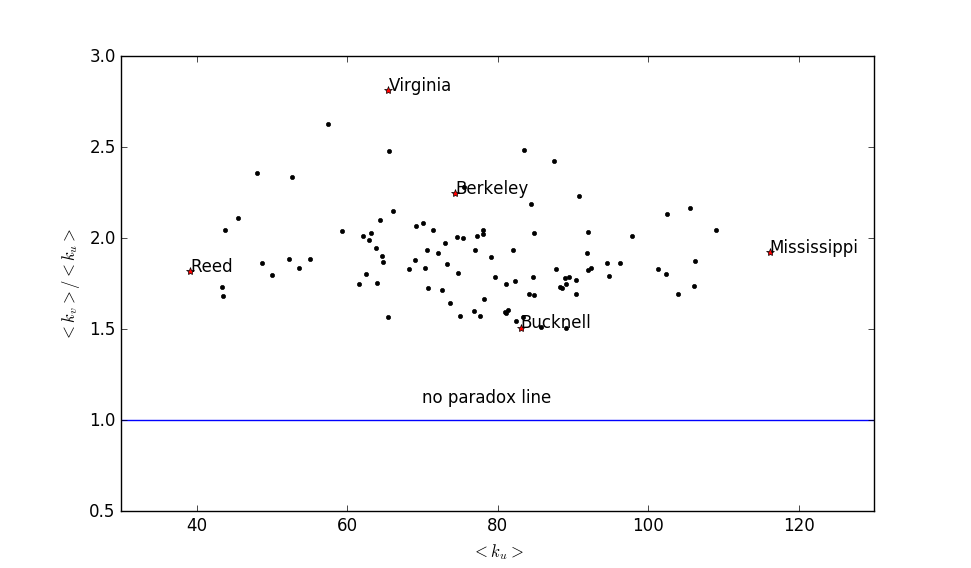
\includegraphics[width=\textwidth]{images/6b1.png}
  \end{minipage}
\end{figure} 

From the above graph we could clearly see that, the friend paradox is observed in all 100 of the FB100 networks  and there is no dependency between size of the paradox (the MND value) and the network’s mean degree.
\bigskip
\item
The friendship paradox in the networks can be attributed the variance in the number of nodes each node is connected to. For eg., there might be a node which might be connected to a large number of nodes in the network, and completely shifts the average neighbour degree. The condition at which friendship paradox is not seen is when all the nodes in the network are connected to equal number of nodes. Mathematically,

$$<k^2>\;\leq\;<k><k>$$

\end{itemize}
\item
The majority illusion is possible only if the vertexes having x=1 as the binary value of their vertex level property have higher mean degrees than the vertexes having x=0. In order to strengthen our intuition for the cause of majority illusion lets look at the below example. \medskip\\Consider a bipartite graph, let the $type\,1$ vertices have the property x=1, and the $type\,2$ have the property x=0 such that numbers of vertices in $type\,1$ is less than the ones in $type\,2$. This satisfies the given fact that the fraction of vertices (q) that exhibit this property is less than 0.5. From problem 3, we know the relation between mean vertices of the two types $c_1\,\&\,c_2$ in a bipartite graph as 
$$c_2 = \dfrac{n_1}{n_2} c_1$$
since the ratio of $\dfrac{n_1}{n_2} < 1$, the mean degree of $c_1$ must be greater than $c_2$ in order to satisfy the above relation, which implies that the nodes possessing this property should have higher degrees and therefore the majority of a node’s neighbors, on average, exhibiting that property will be greater than 0.5 (as the number of nodes in $type\,2$ is greater than $type\,1$). The same reasoning could be generalised to graphs that aren't bipartite.
\newpage
\item

\begin{itemize}
\item
The figure \footnote{The graphs are plotted using only 92 of the total networks. As the code hasn't completed even after running it for full 4 days} below shows two plots, one showing $l_{max}$ versus $network\,size\,(n)$ and another showing $mean\,geodesic\,length <l>$ versus the $size\,of\,largest\,component\,(n)$.

\begin{figure}[H]
  \centering
  \begin{minipage}[b]{\textwidth}
    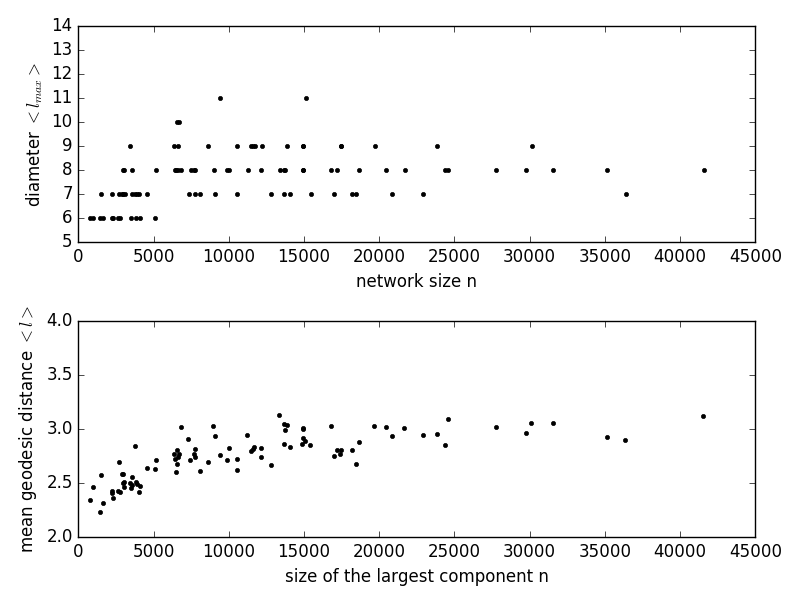
\includegraphics[width=\textwidth]{images/6d1.png}
  \end{minipage}
\end{figure} 
 
 
We could conclude form the $l_{max}$ versus $network\,size\,(n)$  graph above that most of the 100 networks aren't well within the six degrees of separation, this could be attributed to the lower number of connections per person in 2005.
\bigskip
\item
As we know that the average degree of separation between two people is 6 in facebook at present, the diameter of facebook has decreased relative to the these values in 2005. The reason being the number of people in facebook has increased along with the number of connections per individual in recent years. As diameter D with respect to the network size (n) and average degree of a person (k) can be approximated as below,

$$D = \dfrac{\log{n}}{\log{k}}$$

increase in the value of (k) in recent years has kept the diameter D of the network in check and well within a limit, even though the network size has increased considerably.
\end{itemize}
\end{enumerate}


\newpage
\section*{Code - Problem 6B}

\begin{lstlisting}[language=Python, caption=To write data to a file]
import re
import os
import networkx as nx

dataPath = "/home/santa/Dropbox/NAM/Problem Set 1/Data/facebook100txt/"

file = open("/home/santa/Dropbox/NAM/Problem Set 1/Code/data.txt", "w")
for filename in os.listdir(dataPath):
    if filename.endswith(".txt") and not filename.endswith("attr.txt") and 
    						filename.find("readme") == -1:
        lines = [line.rstrip('\n') for line in open(dataPath+filename)]
        
        G = nx.Graph()
        for line in lines:
            vertexes = line.split("\t")
            G.add_edge(vertexes[0], vertexes[1])
        
        listDegree = []
        for node in G.nodes():
            listDegree.append(G.degree(node))
        
        average_degree = sum(listDegree) / (1.0 * G.number_of_nodes())
        average_squared_degree = sum([i ** 2 for i in listDegree]) / 
        						(1.0 * G.number_of_nodes())
        mean_neighbour_degree = average_squared_degree / (1.0 * average_degree)
        name = filename[:re.search("\d", filename).start()]
        file.write(name + "," + str(average_degree) + "," + 
        			str(mean_neighbour_degree/(1.0 * average_degree)) + "\n")
file.close()
\end{lstlisting}
\bigskip

\begin{lstlisting}[language=Python, caption=To plot the data]
import matplotlib.pyplot as plt

filename = "/home/santa/Dropbox/NAM/Problem Set 1/Code/data.txt"
lines = [line.rstrip('\n') for line in open(filename)]
names = ["Reed","Bucknell", "Mississippi", "Virginia", "Berkeley"]

for line in lines:
    pts = line.split(",")
    if pts[0] in names:
        plt.annotate(pts[0], xy=(float(pts[1]),float(pts[2])))
        plt.plot(float(pts[1]),float(pts[2]),'*',color='red')
    else:
        plt.plot(float(pts[1]),float(pts[2]),'.',color='black')

plt.annotate("no paradox line",xy=(70,1.1))
plt.plot([30,130],[1,1])
plt.axis([30,130,0.5,3])
plt.xlabel(r'$<k_u>$')
plt.ylabel(r'$<k_v>/<k_u>$')
plt.show()
\end{lstlisting}

\newpage
\section*{Code - Problem 6D}

\begin{lstlisting}[language=Python, caption=To write data to a file]

import os
import re
import networkx as nx

dataPath = "/home/santa/Dropbox/NAM/Problem Set 1/Data/facebook100txt/"
for filename in os.listdir(dataPath):
    if filename.endswith(".txt") and not filename.endswith("attr.txt") and 
    						filename.find("readme") == -1:
        print filename
        lines = [line.rstrip('\n') for line in open(dataPath+filename)]
        G = nx.Graph()
        for line in lines:
            vertexes = line.split("\t")
            G.add_edge(vertexes[0], vertexes[1])
        
        graphs = sorted(nx.connected_component_subgraphs(G), key=len, reverse=True)
        largest_component = graphs[0]
        n = G.number_of_nodes()
        n_comp = largest_component.number_of_nodes()
        diameter = nx.diameter(largest_component)
        mean_length = nx.average_shortest_path_length(largest_component)
        
        name = filename[:re.search("\d", filename).start()]
        file = open("/home/santa/Dropbox/NAM/Problem Set 1/Code/ec.txt", "a")
        file.write(name + "," + str(diameter) + "," + str(n) + "," + str(mean_length) + 
        					"," + str(n_comp) + "\n")
        file.close()
\end{lstlisting}

\bigskip
\begin{lstlisting}[language=Python, caption=To plot the data]
import matplotlib.pyplot as plt

filename = "/home/santa/Dropbox/NAM/Problem Set 1/Code/ec.txt"
lines = [line.rstrip('\n') for line in open(filename)]

plt.subplot(211)
for line in lines:
    pts = line.split(",")
    plt.plot(float(pts[2]),float(pts[1]),'.',color='black')

plt.axis([0,45000,5,14])
plt.ylabel(r'diameter $<l_{max}>$')
plt.xlabel('network size n')

plt.subplot(212)
for line in lines:
    pts = line.split(",")
    plt.plot(float(pts[4]),float(pts[3]),'.',color='black')

plt.axis([0,45000,2,4])
plt.ylabel(r'mean geodesic distance $<l>$')
plt.xlabel('size of the largest component n')

plt.tight_layout()
plt.show()
\end{lstlisting}

\end{document}
